\documentclass[aspectratio=169,12pt]{beamer}

% Theme and colors
\usetheme{Madrid}
\usecolortheme{whale}
\setbeamertemplate{navigation symbols}{}
\setbeamertemplate{footline}[frame number]

% Packages
\usepackage{amsmath,amssymb}
\usepackage{graphicx}
\usepackage{tikz}
\usetikzlibrary{shapes,arrows,positioning,calc,matrix,patterns}
\usepackage{booktabs}
\usepackage{array}
\usepackage{multirow}
\usepackage{xcolor}
\usepackage{hyperref}

% Custom colors
\definecolor{codegreen}{rgb}{0,0.6,0}
\definecolor{codepurple}{rgb}{0.58,0,0.82}
\definecolor{darkblue}{rgb}{0,0,0.7}
\definecolor{waveblue}{rgb}{0.1,0.4,0.8}

% Title information
\title[Digital Audio \& Compression]{Digital Audio, Lossless \& Lossy Compression,\\and Audio Coding}
\subtitle{From Sound Waves to MP3}
\author[Mahesh C]{\textbf{Mahesh C}\\FISAT}
\institute{Federal Institute of Science and Technology (FISAT)\\Multimedia Technology Class}
\date{\today}

\begin{document}

\begin{frame}
    \titlepage
    \begin{center}
        \small Based on: Li \& Drew, \textit{Fundamentals of Multimedia}, Pearson 2004
    \end{center}
\end{frame}

\begin{frame}{Outline}
    \tableofcontents
\end{frame}


%==============================================================================
\section{Basics of Digital Audio}
%==============================================================================

\begin{frame}{What is Sound?}
    \begin{columns}
        \begin{column}{0.55\textwidth}
            \textbf{Sound is a pressure wave} travelling through air.
            \begin{itemize}
                \item Vibrating object pushes air molecules
                \item Creates alternating high/low pressure regions
                \item Our eardrums vibrate in response
                \item Brain interprets vibrations as sound
            \end{itemize}
            
            \vspace{0.3cm}
            \textbf{Key properties:}
            \begin{itemize}
                \item \textbf{Frequency} (Hz) --- pitch (low/high)
                \item \textbf{Amplitude} --- loudness (quiet/loud)
                \item \textbf{Timbre} --- tone colour (guitar vs piano)
            \end{itemize}
        \end{column}
        \begin{column}{0.4\textwidth}
            \begin{center}
                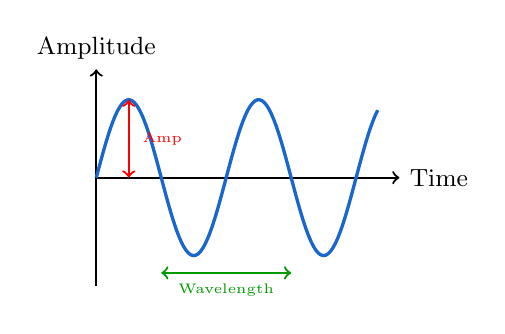
\begin{tikzpicture}[scale=0.55]
                    \draw[->,thick] (0,0) -- (7,0) node[right]{\small Time};
                    \draw[->,thick] (0,-2.5) -- (0,2.5) node[above]{\small Amplitude};
                    \draw[waveblue, very thick, domain=0:6.5, samples=120]
                        plot(\x, {1.8*sin(120*\x)});
                    % labels
                    \draw[<->,red,thick] (0.75,0) -- (0.75,1.8);
                    \node[red,right] at (0.85,0.9) {\tiny Amp};
                    \draw[<->,codegreen,thick] (1.5,-2.2) -- (4.5,-2.2);
                    \node[codegreen] at (3,-2.6) {\tiny Wavelength};
                \end{tikzpicture}
            \end{center}
        \end{column}
    \end{columns}
\end{frame}

\begin{frame}{Human Hearing Range}
    \begin{center}
        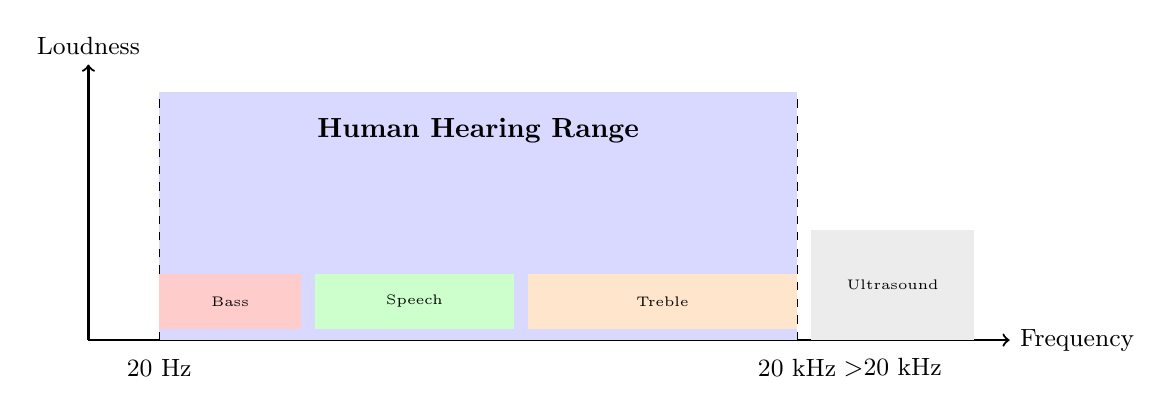
\begin{tikzpicture}[xscale=0.9, yscale=0.7]
            % axis
            \draw[->,thick] (0,0) -- (13,0) node[right]{\small Frequency};
            \draw[->,thick] (0,0) -- (0,5) node[above]{\small Loudness};
            % ranges
            \fill[blue!15] (1,0) rectangle (10,4.5);
            \draw[dashed] (1,0) -- (1,4.5);
            \draw[dashed] (10,0) -- (10,4.5);
            \node at (1,-0.5) {\small 20 Hz};
            \node at (10,-0.5) {\small 20 kHz};
            \node at (5.5,3.8) {\textbf{Human Hearing Range}};
            % sub-ranges
            \fill[red!20] (1,0.2) rectangle (3,1.2);
            \node at (2,0.7) {\tiny Bass};
            \fill[green!20] (3.2,0.2) rectangle (6,1.2);
            \node at (4.6,0.7) {\tiny Speech};
            \fill[orange!20] (6.2,0.2) rectangle (10,1.2);
            \node at (8.1,0.7) {\tiny Treble};
            % ultrasound
            \fill[gray!15] (10.2,0) rectangle (12.5,2);
            \node at (11.35,1) {\tiny Ultrasound};
            \node at (11.35,-0.5) {\small $>$20 kHz};
        \end{tikzpicture}
    \end{center}
    
    \vspace{0.2cm}
    \begin{itemize}
        \item Speech occupies roughly 300 Hz -- 3400 Hz (telephone band)
        \item Music spans the full 20 Hz -- 20 kHz range
        \item Sensitivity peaks around 2--5 kHz (where speech consonants live)
    \end{itemize}
\end{frame}

\begin{frame}{Digitization of Sound: Three Steps}
    \begin{center}
        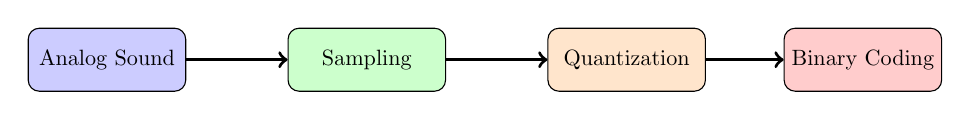
\begin{tikzpicture}[scale=0.6, every node/.style={scale=0.8}]
            \node[draw, fill=blue!20, rounded corners, minimum width=2.5cm, minimum height=1cm] (a) at (0,0) {Analog Sound};
            \node[draw, fill=green!20, rounded corners, minimum width=2.5cm, minimum height=1cm] (s) at (5.5,0) {Sampling};
            \node[draw, fill=orange!20, rounded corners, minimum width=2.5cm, minimum height=1cm] (q) at (11,0) {Quantization};
            \node[draw, fill=red!20, rounded corners, minimum width=2.5cm, minimum height=1cm] (c) at (16,0) {Binary Coding};
            \draw[->,very thick] (a) -- (s);
            \draw[->,very thick] (s) -- (q);
            \draw[->,very thick] (q) -- (c);
        \end{tikzpicture}
    \end{center}
    
    \vspace{0.3cm}
    \begin{columns}
        \begin{column}{0.33\textwidth}
            \textbf{1. Sampling}
            
            Measure the wave at regular intervals.
            
            \textit{How often?}
        \end{column}
        \begin{column}{0.33\textwidth}
            \textbf{2. Quantization}
            
            Round each measurement to the nearest allowed level.
            
            \textit{How precise?}
        \end{column}
        \begin{column}{0.33\textwidth}
            \textbf{3. Binary Coding}
            
            Represent each quantized value as a binary number.
            
            \textit{How many bits?}
        \end{column}
    \end{columns}
\end{frame}


\begin{frame}{Sampling and the Nyquist Theorem}
    \begin{columns}
        \begin{column}{0.55\textwidth}
            \begin{block}{Nyquist--Shannon Sampling Theorem}
                A signal can be perfectly reconstructed if sampled at rate $f_s > 2\,f_{max}$, where $f_{max}$ is the highest frequency present. The rate $2\,f_{max}$ is the \textbf{Nyquist rate}.
            \end{block}
            
            \vspace{0.1cm}
            \textbf{Common sampling rates:}
            \begin{center}
                \small
                \begin{tabular}{l|c|c}
                    \toprule
                    Use & $f_s$ & $f_{max}$ \\
                    \midrule
                    Telephone & 8 kHz & 4 kHz \\
                    AM Radio & 22.05 kHz & 11 kHz \\
                    CD Audio & 44.1 kHz & 22 kHz \\
                    DVD/Studio & 96 kHz & 48 kHz \\
                    \bottomrule
                \end{tabular}
            \end{center}
        \end{column}
        \begin{column}{0.4\textwidth}
            \begin{center}
                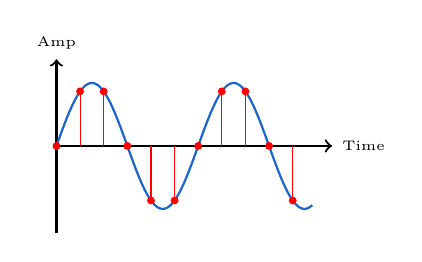
\begin{tikzpicture}[scale=0.5]
                    \draw[->,thick] (0,0) -- (7,0) node[right]{\tiny Time};
                    \draw[->,thick] (0,-2.2) -- (0,2.2) node[above]{\tiny Amp};
                    % continuous
                    \draw[waveblue, thick, domain=0:6.5, samples=100]
                        plot(\x, {1.6*sin(100*\x)});
                    % samples
                    \foreach \x in {0,0.6,...,6.5} {
                        \pgfmathsetmacro{\yval}{1.6*sin(100*\x)}
                        \fill[red] (\x,\yval) circle (0.1);
                        \draw[red,thin] (\x,0) -- (\x,\yval);
                    }
                \end{tikzpicture}
            \end{center}
            {\small Red dots = samples at regular intervals. More samples = better reconstruction.}
        \end{column}
    \end{columns}
\end{frame}

\begin{frame}{Quantization and Bit Depth}
    \begin{columns}
        \begin{column}{0.5\textwidth}
            \textbf{Quantization} maps continuous amplitude to discrete levels.
            
            \vspace{0.3cm}
            \textbf{Bit depth} determines the number of levels:
            \begin{center}
                \begin{tabular}{c|c|c}
                    \toprule
                    Bits & Levels & Use \\
                    \midrule
                    8 & 256 & Telephone \\
                    16 & 65,536 & CD Audio \\
                    24 & 16.7M & Studio \\
                    \bottomrule
                \end{tabular}
            \end{center}
            
            \vspace{0.2cm}
            \textbf{Dynamic range:} $\approx 6$ dB per bit.
            
            16-bit $\rightarrow$ 96 dB (excellent for music).
        \end{column}
        \begin{column}{0.45\textwidth}
            \begin{center}
                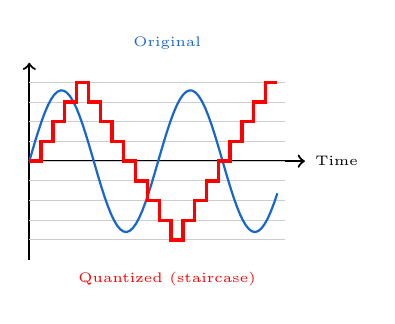
\begin{tikzpicture}[scale=0.5]
                    \draw[->,thick] (0,0) -- (7,0) node[right]{\tiny Time};
                    \draw[->,thick] (0,-2.5) -- (0,2.5);
                    % quantization levels
                    \foreach \y in {-2,-1.5,...,2} {
                        \draw[gray!40,thin] (0,\y) -- (6.5,\y);
                    }
                    % continuous wave
                    \draw[waveblue, thick, domain=0:6.3, samples=80]
                        plot(\x, {1.8*sin(110*\x)});
                    % staircase
                    \draw[red, very thick]
                        (0,0) -- (0.3,0) -- (0.3,0.5) -- (0.6,0.5) --
                        (0.6,1) -- (0.9,1) -- (0.9,1.5) -- (1.2,1.5) --
                        (1.2,2) -- (1.5,2) -- (1.5,1.5) -- (1.8,1.5) --
                        (1.8,1) -- (2.1,1) -- (2.1,0.5) -- (2.4,0.5) --
                        (2.4,0) -- (2.7,0) -- (2.7,-0.5) -- (3,-0.5) --
                        (3,-1) -- (3.3,-1) -- (3.3,-1.5) -- (3.6,-1.5) --
                        (3.6,-2) -- (3.9,-2) -- (3.9,-1.5) -- (4.2,-1.5) --
                        (4.2,-1) -- (4.5,-1) -- (4.5,-0.5) -- (4.8,-0.5) --
                        (4.8,0) -- (5.1,0) -- (5.1,0.5) -- (5.4,0.5) --
                        (5.4,1) -- (5.7,1) -- (5.7,1.5) -- (6,1.5) --
                        (6,2) -- (6.3,2);
                    \node[red] at (3.5,-3) {\tiny Quantized (staircase)};
                    \node[waveblue] at (3.5,3) {\tiny Original};
                \end{tikzpicture}
            \end{center}
        \end{column}
    \end{columns}
\end{frame}

\begin{frame}{Audio Data Rates}
    \textbf{Uncompressed audio data rate:}
    \[
        \text{Rate} = f_s \times \text{bits} \times \text{channels}
    \]
    
    \vspace{0.2cm}
    \begin{center}
        \begin{tabular}{l|c|c|c|c}
            \toprule
            \textbf{Format} & \textbf{Rate} & \textbf{Bits} & \textbf{Ch} & \textbf{Bitrate} \\
            \midrule
            Telephone & 8 kHz & 8 & 1 & 64 kbps \\
            FM Radio & 22 kHz & 16 & 1 & 352 kbps \\
            CD Audio & 44.1 kHz & 16 & 2 & 1,411 kbps \\
            DVD Audio & 96 kHz & 24 & 6 & 13,824 kbps \\
            \bottomrule
        \end{tabular}
    \end{center}
    
    \vspace{0.3cm}
    \begin{alertblock}{The Problem}
        One minute of CD audio = $\frac{1411 \times 60}{8} \approx$ \textbf{10.6 MB}.
        
        A 50-minute album = \textbf{530 MB}. That's why we need compression!
    \end{alertblock}
\end{frame}

%==============================================================================
\section{MIDI}
%==============================================================================

\begin{frame}{Musical Instrument Digital Interface (MIDI)}
    \begin{block}{What is MIDI?}
        MIDI is not audio! It is a \textbf{set of instructions} that tell a synthesizer which notes to play, how loud, and for how long.
    \end{block}
    
    \vspace{0.3cm}
    \begin{columns}
        \begin{column}{0.5\textwidth}
            \textbf{MIDI message example:}
            \begin{center}
                \begin{tabular}{l|l}
                    \toprule
                    Field & Value \\
                    \midrule
                    Note On & Channel 1 \\
                    Pitch & C4 (middle C) \\
                    Velocity & 100 (loud) \\
                    Duration & 500 ms \\
                    Note Off & Channel 1 \\
                    \bottomrule
                \end{tabular}
            \end{center}
        \end{column}
        \begin{column}{0.45\textwidth}
            \textbf{Advantages:}
            \begin{itemize}
                \item Tiny file size (a few KB)
                \item Easy to edit (change tempo, key)
                \item 128 standard instruments
                \item 16 channels simultaneously
            \end{itemize}
            
            \vspace{0.2cm}
            \textbf{Limitation:}
            
            Sound quality depends on the synthesizer, not the file.
        \end{column}
    \end{columns}
\end{frame}

\begin{frame}{MIDI vs Digital Audio}
    \begin{center}
        \begin{tabular}{l|c|c}
            \toprule
            \textbf{Property} & \textbf{MIDI} & \textbf{Digital Audio} \\
            \midrule
            Stores & Instructions & Actual sound \\
            File size (1 min) & $\sim$10 KB & $\sim$10 MB \\
            Edit pitch/tempo & Easy & Difficult \\
            Voice/speech & Cannot represent & Yes \\
            Sound quality & Depends on synth & Fixed at recording \\
            Standard & General MIDI & WAV, AIFF \\
            \bottomrule
        \end{tabular}
    \end{center}
    
    \vspace{0.3cm}
    \begin{block}{Analogy}
        MIDI is like \textbf{sheet music} --- instructions for a musician.
        
        Digital audio is like a \textbf{recording} --- the actual performance captured.
    \end{block}
\end{frame}


%==============================================================================
\section{Lossless Compression Algorithms}
%==============================================================================

\begin{frame}{Why Lossless Compression?}
    \begin{columns}
        \begin{column}{0.5\textwidth}
            \textbf{Lossless = perfect reconstruction.}
            
            Not a single bit is lost.
            
            \vspace{0.3cm}
            \textbf{Used when:}
            \begin{itemize}
                \item Medical data
                \item Legal documents
                \item Software distribution
                \item Archival audio (FLAC)
                \item Text files
            \end{itemize}
        \end{column}
        \begin{column}{0.5\textwidth}
            \textbf{Typical compression ratios:}
            \begin{center}
                \begin{tabular}{l|c}
                    \toprule
                    Data type & Ratio \\
                    \midrule
                    English text & 2:1 -- 3:1 \\
                    Source code & 2:1 -- 4:1 \\
                    Audio (FLAC) & 1.5:1 -- 3:1 \\
                    Images (PNG) & 1.5:1 -- 5:1 \\
                    Random data & $\approx$ 1:1 \\
                    \bottomrule
                \end{tabular}
            \end{center}
            
            \textit{Random data cannot be compressed --- this is a fundamental limit!}
        \end{column}
    \end{columns}
\end{frame}

\begin{frame}{Information Theory: Entropy}
    \begin{block}{Shannon Entropy (1948)}
        The average information content of a source:
        \[
            H(X) = -\sum_{i=1}^{n} p_i \log_2 p_i \quad \text{(bits/symbol)}
        \]
    \end{block}
    
    \vspace{0.2cm}
    \textbf{Entropy sets the absolute limit} on lossless compression.
    
    No lossless code can achieve an average length below $H(X)$.
    
    \vspace{0.3cm}
    \textbf{Quick example:} Source with $P(A)=0.5$, $P(B)=0.25$, $P(C)=0.125$, $P(D)=0.125$
    \[
        H = -(0.5 \cdot (-1) + 0.25 \cdot (-2) + 0.125 \cdot (-3) + 0.125 \cdot (-3)) = 1.75 \text{ bits/symbol}
    \]
    
    \textit{We cannot compress below 1.75 bits per symbol on average.}
\end{frame}

\begin{frame}{Lossless Coding Techniques (Recap)}
    \begin{center}
        \begin{tabular}{l|c|c|c}
            \toprule
            \textbf{Method} & \textbf{Approach} & \textbf{Optimal?} & \textbf{Used in} \\
            \midrule
            Shannon-Fano & Top-down divide & No & Historical \\
            Huffman & Bottom-up merge & Among prefix & JPEG, ZIP \\
            Arithmetic & Interval narrowing & Yes & JPEG2000, H.264 \\
            LZW & Dictionary & Adaptive & GIF, Unix compress \\
            \bottomrule
        \end{tabular}
    \end{center}
    
    \vspace{0.3cm}
    \textbf{Key ideas we covered in earlier lectures:}
    \begin{itemize}
        \item Frequent symbols $\rightarrow$ short codes (variable-length coding)
        \item Prefix-free property ensures unambiguous decoding
        \item Arithmetic coding achieves fractional bits per symbol
        \item Dictionary methods exploit repeated patterns
    \end{itemize}
\end{frame}

%==============================================================================
\section{Distortion Measures \& Rate-Distortion Theory}
%==============================================================================

\begin{frame}{Lossy Compression: Allowing Some Distortion}
    \begin{alertblock}{Key Idea}
        If we accept \textbf{some loss of quality}, we can compress far beyond the entropy limit.
    \end{alertblock}
    
    \vspace{0.3cm}
    \textbf{But how do we measure ``quality loss''?}
    
    \vspace{0.3cm}
    \begin{columns}
        \begin{column}{0.5\textwidth}
            \textbf{Mean Squared Error (MSE):}
            \[
                \text{MSE} = \frac{1}{N}\sum_{i=1}^{N}(x_i - \hat{x}_i)^2
            \]
            Average squared difference between original $x$ and reconstructed $\hat{x}$.
        \end{column}
        \begin{column}{0.5\textwidth}
            \textbf{Signal-to-Noise Ratio (SNR):}
            \[
                \text{SNR} = 10 \log_{10}\frac{\sigma_x^2}{\text{MSE}} \;\text{dB}
            \]
            Higher SNR = better quality.
            
            \vspace{0.2cm}
            \textbf{Typical targets:}
            \begin{itemize}
                \item Speech: 20--30 dB
                \item Music: 60--90 dB
            \end{itemize}
        \end{column}
    \end{columns}
\end{frame}

\begin{frame}{Rate-Distortion Theory}
    \begin{block}{The Fundamental Tradeoff}
        Given a source and a distortion measure, $R(D)$ gives the minimum bit rate to represent the source with distortion $\leq D$.
    \end{block}
    
    \begin{center}
        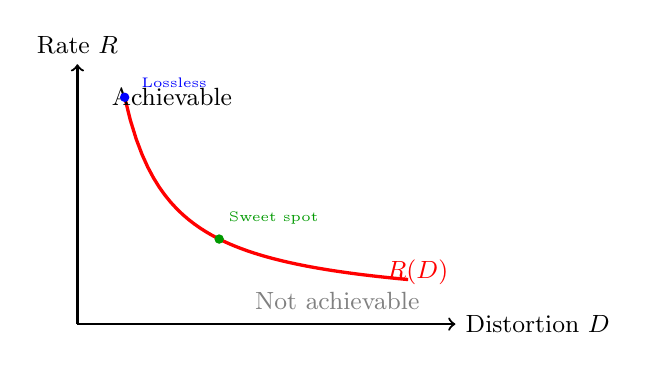
\begin{tikzpicture}[scale=0.6]
            \draw[->,thick] (0,0) -- (8,0) node[right]{\small Distortion $D$};
            \draw[->,thick] (0,0) -- (0,5.5) node[above]{\small Rate $R$};
            % R(D) curve
            \draw[red, very thick, domain=1:7, samples=50]
                plot(\x, {4.5/\x + 0.3});
            \node[red] at (7.2,1.1) {\small $R(D)$};
            % labels
            \node at (2,4.8) {\small Achievable};
            \node[gray] at (5.5,0.5) {\small Not achievable};
            % key points
            \fill[blue] (1,4.8) circle (0.1);
            \node[blue, right] at (1.15,5.1) {\tiny Lossless};
            \fill[codegreen] (3,1.8) circle (0.1);
            \node[codegreen, above right] at (3,1.9) {\tiny Sweet spot};
        \end{tikzpicture}
    \end{center}
    
    \textit{More bits = less distortion. The curve tells us the best possible tradeoff.}
\end{frame}

%==============================================================================
\section{Quantization}
%==============================================================================

\begin{frame}{Quantization: The Core of Lossy Compression}
    \begin{block}{Definition}
        Quantization maps a large (possibly infinite) set of input values to a smaller, finite set of output values. This is inherently lossy.
    \end{block}
    
    \vspace{0.2cm}
    \begin{columns}
        \begin{column}{0.5\textwidth}
            \textbf{Uniform Quantization:}
            \begin{itemize}
                \item Equal-width steps
                \item Simple to implement
            \end{itemize}
            
            \vspace{0.2cm}
            \textbf{Non-uniform Quantization:}
            \begin{itemize}
                \item Smaller steps where signal is common
                \item Better SNR for same bit rate
            \end{itemize}
        \end{column}
        \begin{column}{0.45\textwidth}
            \begin{center}
                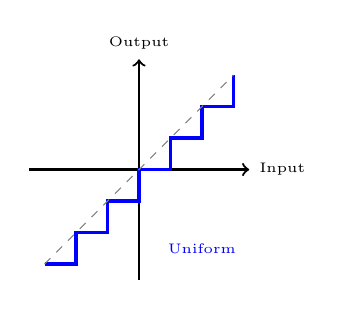
\begin{tikzpicture}[scale=0.4]
                    \draw[->,thick] (-3.5,0) -- (3.5,0) node[right]{\tiny Input};
                    \draw[->,thick] (0,-3.5) -- (0,3.5) node[above]{\tiny Output};
                    % uniform staircase
                    \draw[blue, very thick]
                        (-3,-3) -- (-2,-3) -- (-2,-2) -- (-1,-2) --
                        (-1,-1) -- (0,-1) -- (0,0) -- (1,0) --
                        (1,1) -- (2,1) -- (2,2) -- (3,2) -- (3,3);
                    % ideal line
                    \draw[gray, dashed] (-3,-3) -- (3,3);
                    \node[blue] at (2,-2.5) {\tiny Uniform};
                \end{tikzpicture}
            \end{center}
        \end{column}
    \end{columns}
\end{frame}

\begin{frame}{$\mu$-Law and A-Law Companding}
    \textbf{Used in telephone systems worldwide:}
    
    \vspace{0.3cm}
    \begin{columns}
        \begin{column}{0.5\textwidth}
            \textbf{$\mu$-Law} (North America, Japan):
            \[
                F(x) = \text{sgn}(x)\frac{\ln(1+\mu|x|)}{\ln(1+\mu)}
            \]
            Typically $\mu = 255$.
            
            \vspace{0.3cm}
            \textbf{A-Law} (Europe, rest of world):
            \[
                F(x) = \text{sgn}(x) \times
                \begin{cases}
                    \frac{A|x|}{1+\ln A} & |x| < \frac{1}{A} \\
                    \frac{1+\ln(A|x|)}{1+\ln A} & \text{else}
                \end{cases}
            \]
            Typically $A = 87.6$.
        \end{column}
        \begin{column}{0.45\textwidth}
            \textbf{Why companding?}
            \begin{itemize}
                \item Speech is mostly quiet
                \item Fine steps for quiet sounds
                \item Coarse steps for loud sounds
                \item 8-bit companded $\approx$ 12-bit uniform quality
            \end{itemize}
            
            \vspace{0.3cm}
            \begin{block}{Result}
                Telephone quality at only 64 kbps (8 kHz $\times$ 8 bits).
            \end{block}
        \end{column}
    \end{columns}
\end{frame}

\begin{frame}{Vector Quantization}
    \textbf{Quantize groups of samples together, not one at a time.}
    
    \vspace{0.3cm}
    \begin{columns}
        \begin{column}{0.5\textwidth}
            \textbf{Scalar vs Vector:}
            \begin{itemize}
                \item Scalar: quantize each sample independently
                \item Vector: quantize blocks of $k$ samples as a single unit
                \item Vector is always $\geq$ as efficient as scalar
            \end{itemize}
            
            \vspace{0.2cm}
            \textbf{Codebook:}
            \begin{itemize}
                \item Pre-computed set of representative vectors
                \item Encoder finds closest codebook entry
                \item Sends only the index
            \end{itemize}
        \end{column}
        \begin{column}{0.45\textwidth}
            \begin{center}
                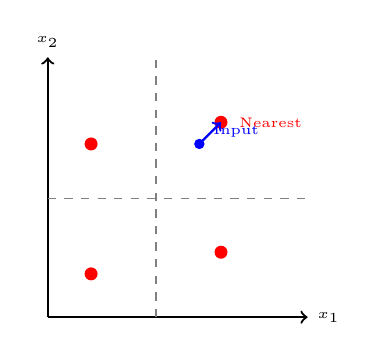
\begin{tikzpicture}[scale=0.55]
                    \draw[->,thick] (0,0) -- (6,0) node[right]{\tiny $x_1$};
                    \draw[->,thick] (0,0) -- (0,6) node[above]{\tiny $x_2$};
                    % codebook points
                    \fill[red] (1,1) circle (0.15);
                    \fill[red] (1,4) circle (0.15);
                    \fill[red] (4,1.5) circle (0.15);
                    \fill[red] (4,4.5) circle (0.15);
                    % input point
                    \fill[blue] (3.5,4) circle (0.12);
                    \node[blue, right] at (3.6,4.3) {\tiny Input};
                    % arrow to nearest
                    \draw[->, blue, thick] (3.5,4) -- (4,4.5);
                    \node[red, right] at (4.2,4.5) {\tiny Nearest};
                    % regions
                    \draw[gray, dashed] (2.5,0) -- (2.5,6);
                    \draw[gray, dashed] (0,2.75) -- (6,2.75);
                \end{tikzpicture}
            \end{center}
            {\small 2D example: four codebook vectors partition the space into four regions.}
        \end{column}
    \end{columns}
\end{frame}


%==============================================================================
\section{Transform Coding \& Wavelets}
%==============================================================================

\begin{frame}{Transform Coding}
    \begin{block}{Core Idea}
        Transform the signal into a different domain where energy is concentrated in a few coefficients. Quantize and code only the important ones.
    \end{block}
    
    \vspace{0.3cm}
    \begin{center}
        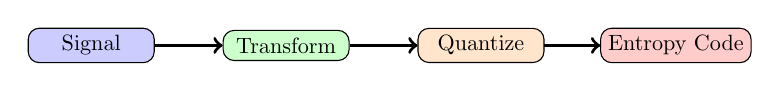
\begin{tikzpicture}[scale=0.55, every node/.style={scale=0.8}]
            \node[draw, fill=blue!20, rounded corners, minimum width=2cm] (sig) at (0,0) {Signal};
            \node[draw, fill=green!20, rounded corners, minimum width=2cm] (trans) at (4.5,0) {Transform};
            \node[draw, fill=orange!20, rounded corners, minimum width=2cm] (quant) at (9,0) {Quantize};
            \node[draw, fill=red!20, rounded corners, minimum width=2cm] (code) at (13.5,0) {Entropy Code};
            \draw[->,very thick] (sig) -- (trans);
            \draw[->,very thick] (trans) -- (quant);
            \draw[->,very thick] (quant) -- (code);
        \end{tikzpicture}
    \end{center}
    
    \vspace{0.3cm}
    \textbf{Common transforms:}
    \begin{itemize}
        \item \textbf{DCT} (Discrete Cosine Transform) --- used in JPEG, MP3
        \item \textbf{DFT} (Discrete Fourier Transform) --- general frequency analysis
        \item \textbf{DWT} (Discrete Wavelet Transform) --- used in JPEG 2000
    \end{itemize}
\end{frame}

\begin{frame}{Why Transforms Help Compression}
    \begin{columns}
        \begin{column}{0.5\textwidth}
            \textbf{Before transform:}
            \begin{itemize}
                \item Energy spread across all samples
                \item Every sample seems important
                \item Hard to decide what to discard
            \end{itemize}
            
            \vspace{0.3cm}
            \textbf{After transform:}
            \begin{itemize}
                \item Energy packed into few coefficients
                \item Most coefficients are near zero
                \item Safe to discard the small ones
            \end{itemize}
        \end{column}
        \begin{column}{0.45\textwidth}
            \begin{center}
                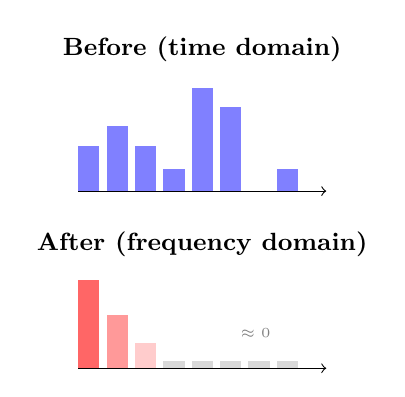
\begin{tikzpicture}[scale=0.45]
                    % Before
                    \node at (3.5,7) {\small\textbf{Before (time domain)}};
                    \foreach \x in {0,...,7} {
                        \pgfmathsetmacro{\h}{1.5+rand*1.5}
                        \fill[blue!50] (\x*0.8, 3) rectangle (\x*0.8+0.6, 3+\h);
                    }
                    \draw[->,thin] (0,3) -- (7,3);
                    
                    % After
                    \node at (3.5,1.5) {\small\textbf{After (frequency domain)}};
                    \fill[red!60] (0,-2) rectangle (0.6,0.5);
                    \fill[red!40] (0.8,-2) rectangle (1.4,-0.5);
                    \fill[red!20] (1.6,-2) rectangle (2.2,-1.3);
                    \foreach \x in {3,...,7} {
                        \fill[gray!30] (\x*0.8, -2) rectangle (\x*0.8+0.6, -1.8);
                    }
                    \draw[->,thin] (0,-2) -- (7,-2);
                    \node[gray] at (5,-1) {\tiny $\approx 0$};
                \end{tikzpicture}
            \end{center}
        \end{column}
    \end{columns}
\end{frame}

\begin{frame}{Wavelet-Based Coding}
    \begin{columns}
        \begin{column}{0.55\textwidth}
            \textbf{Wavelets vs DCT:}
            \begin{itemize}
                \item DCT uses fixed-size blocks (e.g.\ 8$\times$8)
                \item Wavelets use multi-resolution analysis
                \item Better at capturing transients (sharp attacks in audio)
                \item No blocking artifacts
            \end{itemize}
            
            \vspace{0.3cm}
            \textbf{How it works:}
            \begin{enumerate}
                \item Split signal into low-frequency (approximation) and high-frequency (detail) parts
                \item Repeat on the low-frequency part
                \item Creates a multi-level decomposition
            \end{enumerate}
        \end{column}
        \begin{column}{0.4\textwidth}
            \begin{center}
                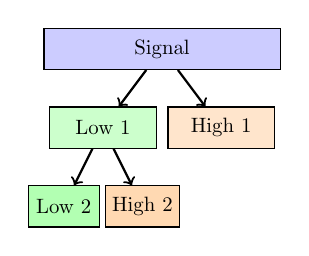
\begin{tikzpicture}[scale=0.5, every node/.style={scale=0.75}]
                    % Level 0
                    \node[draw, fill=blue!20, minimum width=4cm, minimum height=0.7cm] (s) at (0,5) {Signal};
                    % Level 1
                    \node[draw, fill=green!20, minimum width=1.8cm, minimum height=0.7cm] (l1) at (-1.5,3) {Low 1};
                    \node[draw, fill=orange!20, minimum width=1.8cm, minimum height=0.7cm] (h1) at (1.5,3) {High 1};
                    % Level 2
                    \node[draw, fill=green!30, minimum width=1.2cm, minimum height=0.7cm] (l2) at (-2.5,1) {Low 2};
                    \node[draw, fill=orange!30, minimum width=1.2cm, minimum height=0.7cm] (h2) at (-0.5,1) {High 2};
                    % arrows
                    \draw[->,thick] (s) -- (l1);
                    \draw[->,thick] (s) -- (h1);
                    \draw[->,thick] (l1) -- (l2);
                    \draw[->,thick] (l1) -- (h2);
                \end{tikzpicture}
            \end{center}
            
            \vspace{0.2cm}
            {\small Each level halves the frequency resolution and doubles the time resolution.}
        \end{column}
    \end{columns}
\end{frame}

\begin{frame}{Wavelet Packets}
    \begin{block}{Extension of Standard Wavelets}
        Standard wavelets only decompose the low-frequency part at each level. Wavelet packets decompose \textbf{both} low and high frequency parts, giving a richer set of bases.
    \end{block}
    
    \vspace{0.3cm}
    \begin{center}
        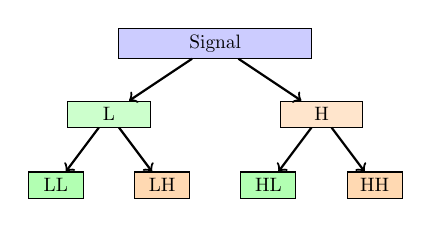
\begin{tikzpicture}[scale=0.45, every node/.style={scale=0.7}]
            % Full tree
            \node[draw, fill=blue!20, minimum width=3.5cm] (s) at (0,5) {Signal};
            
            \node[draw, fill=green!20, minimum width=1.5cm] (l) at (-3,3) {L};
            \node[draw, fill=orange!20, minimum width=1.5cm] (h) at (3,3) {H};
            
            \node[draw, fill=green!30, minimum width=1cm] (ll) at (-4.5,1) {LL};
            \node[draw, fill=orange!30, minimum width=1cm] (lh) at (-1.5,1) {LH};
            \node[draw, fill=green!30, minimum width=1cm] (hl) at (1.5,1) {HL};
            \node[draw, fill=orange!30, minimum width=1cm] (hh) at (4.5,1) {HH};
            
            \draw[->,thick] (s) -- (l);
            \draw[->,thick] (s) -- (h);
            \draw[->,thick] (l) -- (ll);
            \draw[->,thick] (l) -- (lh);
            \draw[->,thick] (h) -- (hl);
            \draw[->,thick] (h) -- (hh);
        \end{tikzpicture}
    \end{center}
    
    \vspace{0.2cm}
    \textbf{Advantage:} The best decomposition tree can be chosen adaptively for each signal, giving better energy compaction than a fixed wavelet decomposition.
    
    \textit{Used in some advanced audio coders and JPEG 2000.}
\end{frame}


%==============================================================================
\section{Audio Compression Techniques}
%==============================================================================

\begin{frame}{Audio Compression: The Landscape}
    \begin{center}
        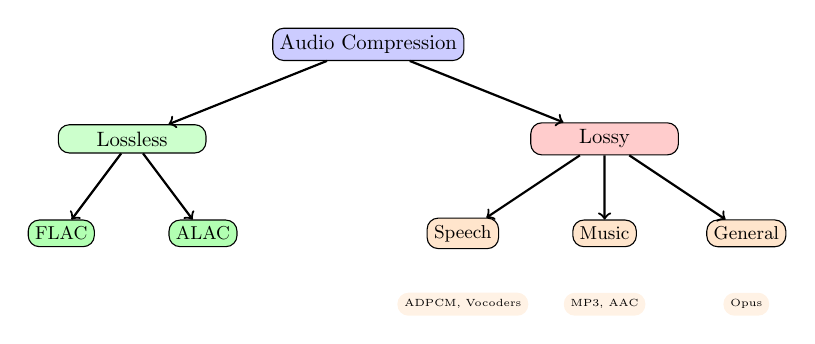
\begin{tikzpicture}[scale=0.6, every node/.style={scale=0.75}]
            % Tree
            \node[draw, fill=blue!20, rounded corners, minimum width=3cm] (root) at (0,5) {Audio Compression};
            
            \node[draw, fill=green!20, rounded corners, minimum width=2.5cm] (loss) at (-5,3) {Lossless};
            \node[draw, fill=red!20, rounded corners, minimum width=2.5cm] (lossy) at (5,3) {Lossy};
            
            \node[draw, fill=green!30, rounded corners] (flac) at (-6.5,1) {\small FLAC};
            \node[draw, fill=green!30, rounded corners] (alac) at (-3.5,1) {\small ALAC};
            
            \node[draw, fill=orange!20, rounded corners] (speech) at (2,1) {\small Speech};
            \node[draw, fill=orange!20, rounded corners] (music) at (5,1) {\small Music};
            \node[draw, fill=orange!20, rounded corners] (gen) at (8,1) {\small General};
            
            \node[fill=orange!10, rounded corners] at (2,-0.5) {\tiny ADPCM, Vocoders};
            \node[fill=orange!10, rounded corners] at (5,-0.5) {\tiny MP3, AAC};
            \node[fill=orange!10, rounded corners] at (8,-0.5) {\tiny Opus};
            
            \draw[->,thick] (root) -- (loss);
            \draw[->,thick] (root) -- (lossy);
            \draw[->,thick] (loss) -- (flac);
            \draw[->,thick] (loss) -- (alac);
            \draw[->,thick] (lossy) -- (speech);
            \draw[->,thick] (lossy) -- (music);
            \draw[->,thick] (lossy) -- (gen);
        \end{tikzpicture}
    \end{center}
\end{frame}

\begin{frame}{ADPCM in Speech Coding}
    \begin{block}{Adaptive Differential Pulse Code Modulation}
        Instead of coding the signal itself, code the \textbf{difference} between the actual sample and a \textbf{prediction} of it.
    \end{block}
    
    \vspace{0.3cm}
    \begin{columns}
        \begin{column}{0.5\textwidth}
            \textbf{How ADPCM works:}
            \begin{enumerate}
                \item Predict next sample from previous ones
                \item Compute prediction error (residual)
                \item Quantize the error (much smaller!)
                \item Adapt step size based on signal
            \end{enumerate}
            
            \vspace{0.2cm}
            \textit{Adjacent speech samples are highly correlated, so the difference is small and needs fewer bits.}
        \end{column}
        \begin{column}{0.45\textwidth}
            \begin{center}
                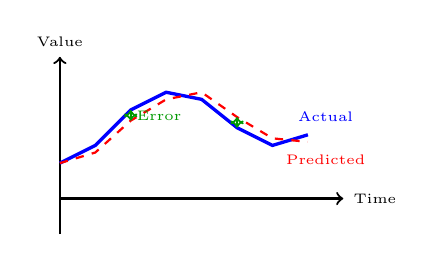
\begin{tikzpicture}[scale=0.45]
                    \draw[->,thick] (0,0) -- (8,0) node[right]{\tiny Time};
                    \draw[->,thick] (0,-1) -- (0,4) node[above]{\tiny Value};
                    % actual signal
                    \draw[blue, very thick] (0,1) -- (1,1.5) -- (2,2.5) -- (3,3) -- (4,2.8) -- (5,2) -- (6,1.5) -- (7,1.8);
                    % predicted
                    \draw[red, thick, dashed] (0,1) -- (1,1.3) -- (2,2.2) -- (3,2.8) -- (4,3) -- (5,2.3) -- (6,1.7) -- (7,1.6);
                    % error arrows
                    \draw[codegreen, <->, thick] (2,2.2) -- (2,2.5);
                    \draw[codegreen, <->, thick] (5,2) -- (5,2.3);
                    \node[blue] at (7.5,2.3) {\tiny Actual};
                    \node[red] at (7.5,1.1) {\tiny Predicted};
                    \node[codegreen] at (2.8,2.35) {\tiny Error};
                \end{tikzpicture}
            \end{center}
            
            G.726 achieves toll-quality speech at \textbf{32 kbps} (half of PCM's 64 kbps).
        \end{column}
    \end{columns}
\end{frame}

\begin{frame}{Vocoders: Modelling the Voice}
    \begin{block}{Vocoder = Voice Coder}
        Instead of coding the waveform, model the \textbf{speech production system} (vocal tract) and transmit only the model parameters.
    \end{block}
    
    \vspace{0.3cm}
    \begin{center}
        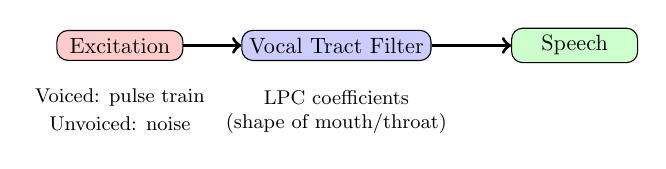
\begin{tikzpicture}[scale=0.55, every node/.style={scale=0.8}]
            % Source
            \node[draw, fill=red!20, rounded corners, minimum width=2cm] (exc) at (0,0) {Excitation};
            % Filter
            \node[draw, fill=blue!20, rounded corners, minimum width=2.5cm] (filt) at (5,0) {Vocal Tract Filter};
            % Output
            \node[draw, fill=green!20, rounded corners, minimum width=2cm] (out) at (10.5,0) {Speech};
            
            \draw[->,very thick] (exc) -- (filt);
            \draw[->,very thick] (filt) -- (out);
            
            % Labels below
            \node at (0,-1.2) {\small Voiced: pulse train};
            \node at (0,-1.8) {\small Unvoiced: noise};
            \node at (5,-1.2) {\small LPC coefficients};
            \node at (5,-1.8) {\small (shape of mouth/throat)};
        \end{tikzpicture}
    \end{center}
    
    \vspace{0.2cm}
    \textbf{Extremely low bitrates:} 2.4 -- 9.6 kbps (vs 64 kbps for PCM).
    
    \textbf{Tradeoff:} Sounds robotic at very low rates. Good for military, satellite.
\end{frame}

\begin{frame}{Waveform vs Model-Based vs Hybrid}
    \begin{center}
        \begin{tabular}{l|c|c|c}
            \toprule
            & \textbf{Waveform} & \textbf{Vocoder} & \textbf{Hybrid} \\
            \midrule
            Approach & Code signal & Code model & Both \\
            Example & PCM, ADPCM & LPC vocoder & CELP \\
            Bitrate & 16--64 kbps & 2.4--4.8 kbps & 4.8--16 kbps \\
            Quality & Natural & Robotic & Good \\
            Non-speech & Good & Poor & Fair \\
            \bottomrule
        \end{tabular}
    \end{center}
    
    \vspace{0.3cm}
    \begin{block}{CELP (Code-Excited Linear Prediction)}
        The dominant speech coding paradigm today. Used in GSM, 3G, 4G, VoLTE.
        
        Combines LPC modelling with a codebook of excitation patterns.
        
        Achieves near-toll quality at 8--13 kbps.
    \end{block}
\end{frame}

%==============================================================================
\section{Psychoacoustics}
%==============================================================================

\begin{frame}{Psychoacoustics: What You Can't Hear}
    \begin{alertblock}{Key Insight}
        The human ear has limitations. If we know what you \textbf{cannot hear}, we can throw it away and save bits!
    \end{alertblock}
    
    \vspace{0.3cm}
    \textbf{Two main phenomena:}
    
    \vspace{0.2cm}
    \begin{columns}
        \begin{column}{0.5\textwidth}
            \textbf{1. Absolute Threshold of Hearing}
            \begin{itemize}
                \item Minimum loudness to hear a tone
                \item Varies with frequency
                \item Most sensitive at 2--5 kHz
                \item Anything below the threshold is inaudible
            \end{itemize}
        \end{column}
        \begin{column}{0.5\textwidth}
            \textbf{2. Masking}
            \begin{itemize}
                \item A loud sound hides nearby quiet sounds
                \item Frequency masking (simultaneous)
                \item Temporal masking (before/after)
                \item The hidden sounds can be removed!
            \end{itemize}
        \end{column}
    \end{columns}
\end{frame}

\begin{frame}{Absolute Threshold of Hearing}
    \begin{center}
        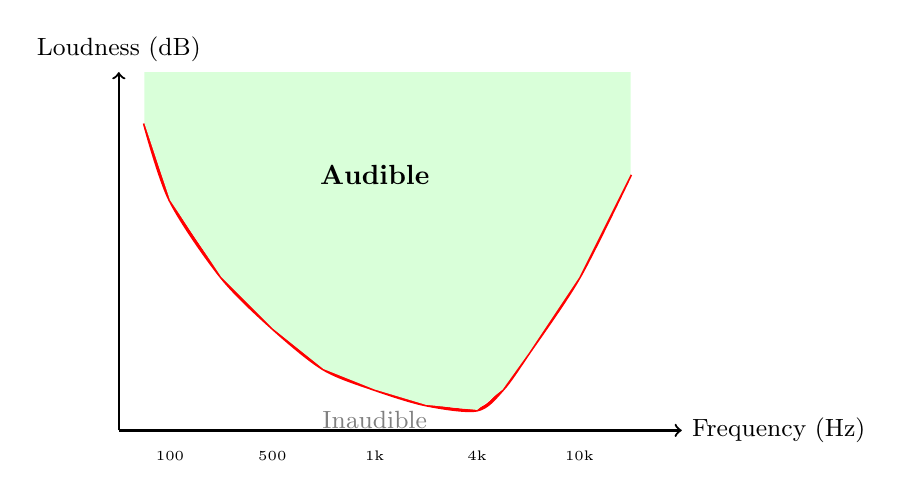
\begin{tikzpicture}[scale=0.65]
            \draw[->,thick] (0,0) -- (11,0) node[right]{\small Frequency (Hz)};
            \draw[->,thick] (0,0) -- (0,7) node[above]{\small Loudness (dB)};
            
            % Frequency labels
            \node at (1,-0.5) {\tiny 100};
            \node at (3,-0.5) {\tiny 500};
            \node at (5,-0.5) {\tiny 1k};
            \node at (7,-0.5) {\tiny 4k};
            \node at (9,-0.5) {\tiny 10k};
            
            % Threshold curve (simplified)
            \draw[red, very thick, smooth]
                plot coordinates {(0.5,6) (1,4.5) (2,3) (3,2) (4,1.2) (5,0.8) (6,0.5) (7,0.4) (7.5,0.8) (8,1.5) (9,3) (10,5)};
            
            \node[red] at (8.5,5.5) {\small Threshold};
            
            % Regions
            \fill[green!15] (0.5,6) -- (1,4.5) -- (2,3) -- (3,2) -- (4,1.2) -- (5,0.8) -- (6,0.5) -- (7,0.4) -- (7.5,0.8) -- (8,1.5) -- (9,3) -- (10,5) -- (10,7) -- (0.5,7) -- cycle;
            
            \node at (5,5) {\textbf{Audible}};
            \node[gray] at (5,0.2) {\small Inaudible};
        \end{tikzpicture}
    \end{center}
    
    \vspace{0.1cm}
    Sounds below the red curve are \textbf{inaudible} --- no need to encode them!
\end{frame}

\begin{frame}{Frequency Masking}
    \begin{center}
        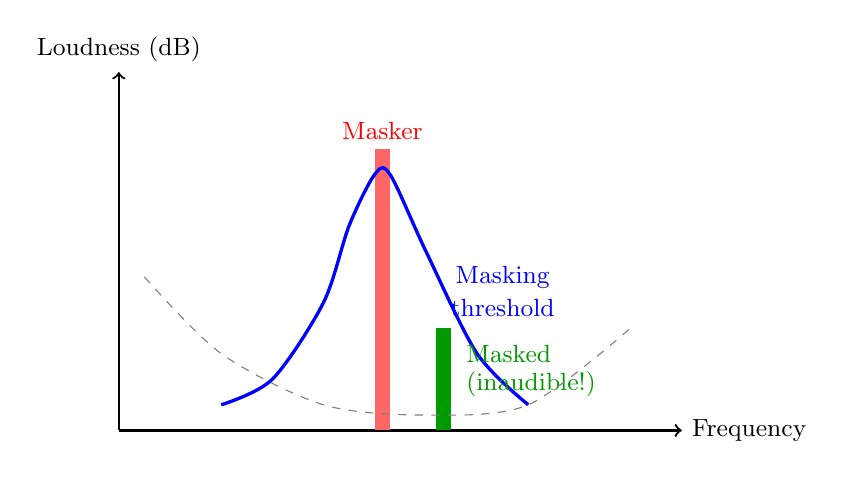
\begin{tikzpicture}[scale=0.65]
            \draw[->,thick] (0,0) -- (11,0) node[right]{\small Frequency};
            \draw[->,thick] (0,0) -- (0,7) node[above]{\small Loudness (dB)};
            
            % Masker tone
            \fill[red!60] (5,0) -- (5,5.5) -- (5.3,5.5) -- (5.3,0) -- cycle;
            \node[red, above] at (5.15,5.5) {\small Masker};
            
            % Masking threshold (spread)
            \draw[blue, very thick, smooth]
                plot coordinates {(2,0.5) (3,1) (4,2.5) (4.5,4) (5,5) (5.3,5) (6,3.5) (7,1.5) (8,0.5)};
            \node[blue] at (7.5,3) {\small Masking};
            \node[blue] at (7.5,2.4) {\small threshold};
            
            % Masked tone
            \fill[codegreen] (6.2,0) -- (6.2,2) -- (6.5,2) -- (6.5,0) -- cycle;
            \node[codegreen, right] at (6.6,1.5) {\small Masked};
            \node[codegreen, right] at (6.6,0.9) {\small (inaudible!)};
            
            % Quiet threshold
            \draw[gray, dashed, smooth]
                plot coordinates {(0.5,3) (2,1.5) (4,0.5) (6,0.3) (8,0.5) (10,2)};
        \end{tikzpicture}
    \end{center}
    
    \vspace{0.2cm}
    A loud tone at one frequency raises the hearing threshold for nearby frequencies. Quiet tones near a loud one become \textbf{inaudible} and can be discarded.
\end{frame}

\begin{frame}{Temporal Masking}
    \begin{center}
        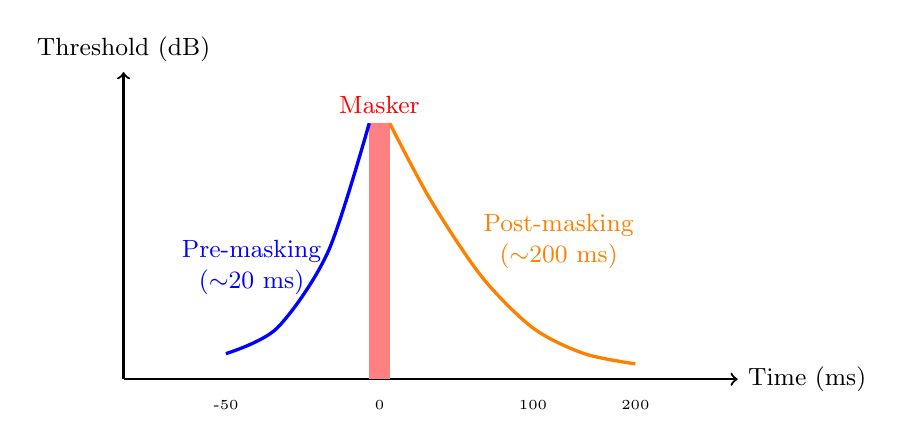
\begin{tikzpicture}[scale=0.65]
            \draw[->,thick] (0,0) -- (12,0) node[right]{\small Time (ms)};
            \draw[->,thick] (0,0) -- (0,6) node[above]{\small Threshold (dB)};
            
            % Time labels
            \node at (2,-0.5) {\tiny -50};
            \node at (5,-0.5) {\tiny 0};
            \node at (8,-0.5) {\tiny 100};
            \node at (10,-0.5) {\tiny 200};
            
            % Masker
            \fill[red!50] (4.8,0) rectangle (5.2,5);
            \node[red, above] at (5,5) {\small Masker};
            
            % Pre-masking
            \draw[blue, very thick, smooth]
                plot coordinates {(2,0.5) (3,1) (4,2.5) (4.8,5)};
            \node[blue] at (2.5,2.5) {\small Pre-masking};
            \node[blue] at (2.5,1.9) {\small ($\sim$20 ms)};
            
            % Post-masking
            \draw[orange, very thick, smooth]
                plot coordinates {(5.2,5) (6,3.5) (7,2) (8,1) (9,0.5) (10,0.3)};
            \node[orange] at (8.5,3) {\small Post-masking};
            \node[orange] at (8.5,2.4) {\small ($\sim$200 ms)};
        \end{tikzpicture}
    \end{center}
    
    \vspace{0.2cm}
    A loud sound masks quiet sounds that occur \textbf{just before} (pre-masking, $\sim$20 ms) and \textbf{after} it (post-masking, $\sim$200 ms).
\end{frame}

%==============================================================================
\section{MPEG Audio (MP3)}
%==============================================================================

\begin{frame}{MPEG Audio: Three Layers}
    \begin{center}
        \begin{tabular}{l|c|c|c}
            \toprule
            & \textbf{Layer I} & \textbf{Layer II} & \textbf{Layer III (MP3)} \\
            \midrule
            Complexity & Low & Medium & High \\
            Quality at 128 kbps & Fair & Good & Excellent \\
            Typical bitrate & 384 kbps & 192 kbps & 128 kbps \\
            Compression ratio & 4:1 & 8:1 & 12:1 \\
            Use & DCC tape & DAB radio & Internet, players \\
            \bottomrule
        \end{tabular}
    \end{center}
    
    \vspace{0.3cm}
    \begin{block}{MP3 = MPEG-1 Audio Layer III}
        The most popular audio format in history. Achieves near-CD quality at 128--192 kbps (vs 1411 kbps for CD).
        
        \textbf{Key idea:} Combine transform coding with psychoacoustic modelling.
    \end{block}
\end{frame}

\begin{frame}{MP3 Encoder Pipeline}
    \begin{center}
        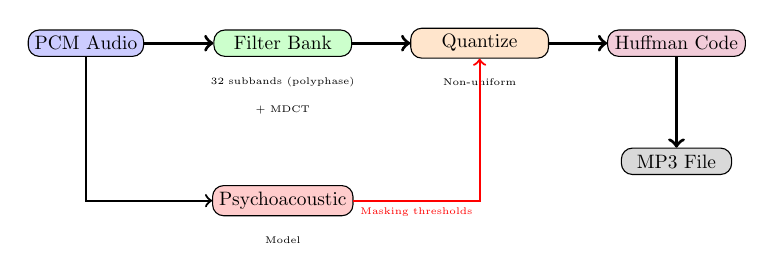
\begin{tikzpicture}[scale=0.5, every node/.style={scale=0.7}]
            % Input
            \node[draw, fill=blue!20, rounded corners, minimum width=2cm] (pcm) at (0,3) {PCM Audio};
            
            % Filter bank
            \node[draw, fill=green!20, rounded corners, minimum width=2.5cm] (fb) at (5,3) {Filter Bank};
            \node at (5,2) {\tiny 32 subbands (polyphase)};
            \node at (5,1.3) {\tiny + MDCT};
            
            % Psychoacoustic
            \node[draw, fill=red!20, rounded corners, minimum width=2.5cm] (psy) at (5,-1) {Psychoacoustic};
            \node at (5,-2) {\tiny Model};
            
            % Quantize
            \node[draw, fill=orange!20, rounded corners, minimum width=2.5cm] (quant) at (10,3) {Quantize};
            \node at (10,2) {\tiny Non-uniform};
            
            % Huffman
            \node[draw, fill=purple!20, rounded corners, minimum width=2.5cm] (huff) at (15,3) {Huffman Code};
            
            % Bitstream
            \node[draw, fill=gray!30, rounded corners, minimum width=2cm] (out) at (15,0) {MP3 File};
            
            % Arrows
            \draw[->,very thick] (pcm) -- (fb);
            \draw[->,very thick] (fb) -- (quant);
            \draw[->,very thick] (quant) -- (huff);
            \draw[->,very thick] (huff) -- (out);
            \draw[->,thick] (pcm) |- (psy);
            \draw[->,thick, red] (psy) -| (quant) node[near start, below] {\tiny Masking thresholds};
        \end{tikzpicture}
    \end{center}
    
    \vspace{0.3cm}
    \textbf{Key steps:}
    \begin{enumerate}
        \item \textbf{Filter bank:} Split audio into 576 frequency bands (32 subbands $\times$ 18 MDCT)
        \item \textbf{Psychoacoustic model:} Calculate masking thresholds for each band
        \item \textbf{Quantize:} Allocate bits per band --- more bits where ear is sensitive
        \item \textbf{Huffman code:} Lossless compression of quantized values
    \end{enumerate}
\end{frame}

\begin{frame}{How MP3 Uses Psychoacoustics}
    \textbf{The psychoacoustic model drives everything:}
    
    \vspace{0.3cm}
    \begin{enumerate}
        \item Analyze the audio frame (1152 samples $\approx$ 26 ms)
        \item Compute the power spectrum via FFT
        \item Identify tonal (sinusoidal) and noise-like components
        \item Calculate masking thresholds for each critical band
        \item Determine the \textbf{Signal-to-Mask Ratio (SMR)} per band
        \item Allocate bits: bands with high SMR get more bits
    \end{enumerate}
    
    \vspace{0.3cm}
    \begin{block}{The Magic}
        Quantization noise is shaped to stay \textbf{below the masking threshold}.
        
        The noise is there, but you \textbf{cannot hear it}!
        
        This is called \textbf{noise shaping} or \textbf{perceptual coding}.
    \end{block}
\end{frame}

\begin{frame}{MP3 Quality Comparison}
    \begin{center}
        \small
        \begin{tabular}{l|c|c|l}
            \toprule
            \textbf{Bitrate} & \textbf{Ratio} & \textbf{Size/min} & \textbf{Quality} \\
            \midrule
            320 kbps & 4.4:1 & 2.4 MB & Transparent \\
            192 kbps & 7.3:1 & 1.4 MB & Very good \\
            128 kbps & 11:1 & 960 KB & Good (most common) \\
            64 kbps & 22:1 & 480 KB & Noticeable artifacts \\
            \bottomrule
        \end{tabular}
    \end{center}
    
    \vspace{0.2cm}
    \begin{columns}
        \begin{column}{0.55\textwidth}
            \textbf{A 50-minute CD album:}
            \begin{itemize}
                \item Uncompressed WAV: \textbf{530 MB}
                \item MP3 at 128 kbps: \textbf{48 MB} (11$\times$ smaller)
                \item MP3 at 320 kbps: \textbf{120 MB} (4.4$\times$ smaller)
            \end{itemize}
        \end{column}
        \begin{column}{0.4\textwidth}
            \begin{alertblock}{The MP3 Revolution}
                Made digital music distribution practical. Napster, iPod, and the entire streaming era followed.
            \end{alertblock}
        \end{column}
    \end{columns}
\end{frame}

\begin{frame}{Beyond MP3: Modern Audio Codecs}
    \begin{center}
        \small
        \begin{tabular}{l|c|c|l}
            \toprule
            \textbf{Codec} & \textbf{Year} & \textbf{Type} & \textbf{Used in} \\
            \midrule
            MP3 & 1993 & Lossy & Legacy, portable players \\
            AAC & 1997 & Lossy & iTunes, YouTube \\
            FLAC & 2001 & Lossless & Archival, audiophiles \\
            Opus & 2012 & Both & Discord, WhatsApp, WebRTC \\
            \bottomrule
        \end{tabular}
    \end{center}
    
    \vspace{0.2cm}
    \begin{columns}
        \begin{column}{0.5\textwidth}
            \textbf{Opus --- The Modern Champion:}
            \begin{itemize}
                \item Speech and music in one codec
                \item 6 kbps (speech) to 510 kbps (music)
                \item Lower latency than MP3
                \item Open and royalty-free
            \end{itemize}
        \end{column}
        \begin{column}{0.45\textwidth}
            \begin{block}{Takeaway}
                Opus beats MP3 and AAC at every bitrate. It is the recommended codec for real-time communication and streaming today.
            \end{block}
        \end{column}
    \end{columns}
\end{frame}

%==============================================================================
\section{Summary}
%==============================================================================

\begin{frame}{Key Takeaways}
    \begin{enumerate}
        \item \textbf{Digitization:} Sampling (Nyquist), quantization (bit depth), binary coding
        
        \item \textbf{MIDI:} Instructions, not audio --- tiny files, editable, synth-dependent
        
        \item \textbf{Lossless compression:} Entropy is the limit; Huffman, arithmetic, LZW
        
        \item \textbf{Lossy compression:} Rate-distortion tradeoff; quantization is the core
        
        \item \textbf{Transforms:} DCT and wavelets concentrate energy for efficient coding
        
        \item \textbf{Speech coding:} ADPCM (prediction), vocoders (modelling), CELP (hybrid)
        
        \item \textbf{Psychoacoustics:} Masking and hearing thresholds let us discard inaudible data
        
        \item \textbf{MP3:} Filter bank + psychoacoustic model + quantization + Huffman = 11:1 compression with near-CD quality
    \end{enumerate}
\end{frame}

\begin{frame}
    \begin{center}
        \Huge{\textbf{Thank You!}}
        
        \vspace{1cm}
        \Large{Questions?}
        
        \vspace{1.5cm}
        \normalsize
        \textit{``If you can't hear it, don't waste bits on it.''}
        
        \vspace{0.3cm}
        --- The philosophy behind perceptual audio coding
    \end{center}
\end{frame}

\end{document}
